% Generated by misc/paper_b/tools/build_figures.py from NUMBERS_TABLE.csv. Do not edit.
% Retrospective item screen (registered A, permutation null, direct contrasts)
\documentclass[border=3pt]{standalone}
\usepackage[T1]{fontenc}
\usepackage{lmodern,amsmath,xcolor}
\usepackage{tikz}
\pdftrailerid{}
\definecolor{cA}{HTML}{0072B2}% blue
\definecolor{cB}{HTML}{D55E00}% vermillion
\definecolor{cC}{HTML}{009E73}% green
\definecolor{cD}{HTML}{CC79A7}% purple
\definecolor{cG}{HTML}{6B6B6B}% grey
\definecolor{cS}{HTML}{3A3A3A}
\definecolor{zebra}{HTML}{F1F1F1}
\definecolor{gridc}{HTML}{C8C8C8}
\newcommand{\Px}{0}\newcommand{\Pmin}{0}\newcommand{\Psc}{1}
% \setpanel{x0 cm}{data value at x0}{cm per data unit}: every data x below is x0 + (v - vmin) * scale.
\newcommand{\setpanel}[3]{\renewcommand{\Px}{#1}\renewcommand{\Pmin}{#2}\renewcommand{\Psc}{#3}}
\newcommand{\XX}[1]{\fpeval{\Px+((#1)-(\Pmin))*\Psc}}
% markers: o filled circle, s filled square, d hollow diamond, t filled triangle, h hollow circle, q hollow square
\newcommand{\mk}[4]{% style colour x y
  \ifx#1o\fill[#2] (#3,#4) circle (0.095);\fi
  \ifx#1h\draw[#2,fill=white,line width=0.7pt] (#3,#4) circle (0.095);\fi
  \ifx#1s\fill[#2] (#3-0.088,#4-0.088) rectangle (#3+0.088,#4+0.088);\fi
  \ifx#1q\draw[#2,fill=white,line width=0.7pt] (#3-0.085,#4-0.085) rectangle (#3+0.085,#4+0.085);\fi
  \ifx#1d\draw[#2,fill=white,line width=0.7pt] (#3,#4+0.125)--(#3+0.125,#4)--(#3,#4-0.125)--(#3-0.125,#4)--cycle;\fi
  \ifx#1t\fill[#2] (#3,#4+0.115)--(#3+0.105,#4-0.085)--(#3-0.105,#4-0.085)--cycle;\fi}
% interval with point: claim, lo, value, hi, y, style, colour, dash(solid|dashed)
\newcommand{\ival}[8]{%
  \edef\xl{\XX{#2}}\edef\xv{\XX{#3}}\edef\xh{\XX{#4}}%
  \draw[#7,line width=0.8pt,#8] (\xl,#5)--(\xh,#5);
  \draw[#7,line width=0.8pt] (\xl,#5-0.055)--(\xl,#5+0.055);
  \draw[#7,line width=0.8pt] (\xh,#5-0.055)--(\xh,#5+0.055);
  \mk{#6}{#7}{\xv}{#5}}
% point only
\newcommand{\pval}[5]{\edef\xv{\XX{#2}}\mk{#4}{#5}{\xv}{#3}}
% stem from the panel zero to the value, with marker: claim, value, y, style, colour
\newcommand{\lval}[5]{\edef\xv{\XX{#2}}\edef\xz{\XX{0}}%
  \draw[#5,line width=0.8pt] (\xz,#3)--(\xv,#3);\mk{#4}{#5}{\xv}{#3}}
% vertical reference line at a data value: claim, value, y0, y1, colour
\newcommand{\vref}[5]{\edef\xv{\XX{#2}}\draw[#5,dashed,line width=0.8pt] (\xv,#3)--(\xv,#4);}
% a printed number tied to a table cell: claim, field, printed, prefix, suffix, x, y, anchor, background fill
\newcommand{\lbl}[9]{\node[anchor=#8,fill=#9,inner sep=1pt,font=\footnotesize] at (#6,#7) {#4#3#5};}
% a printed value with its interval: claim, printed value, printed lo, printed hi, x, y, anchor
\newcommand{\lblci}[7]{\node[anchor=#7,inner sep=0pt,font=\footnotesize] at (#5,#6) {#2\,[#3, #4]};}
% free text (no data)
\newcommand{\txt}[4]{\node[anchor=#3,inner sep=0pt,font=#4] at (#1) {#2};}
\begin{document}
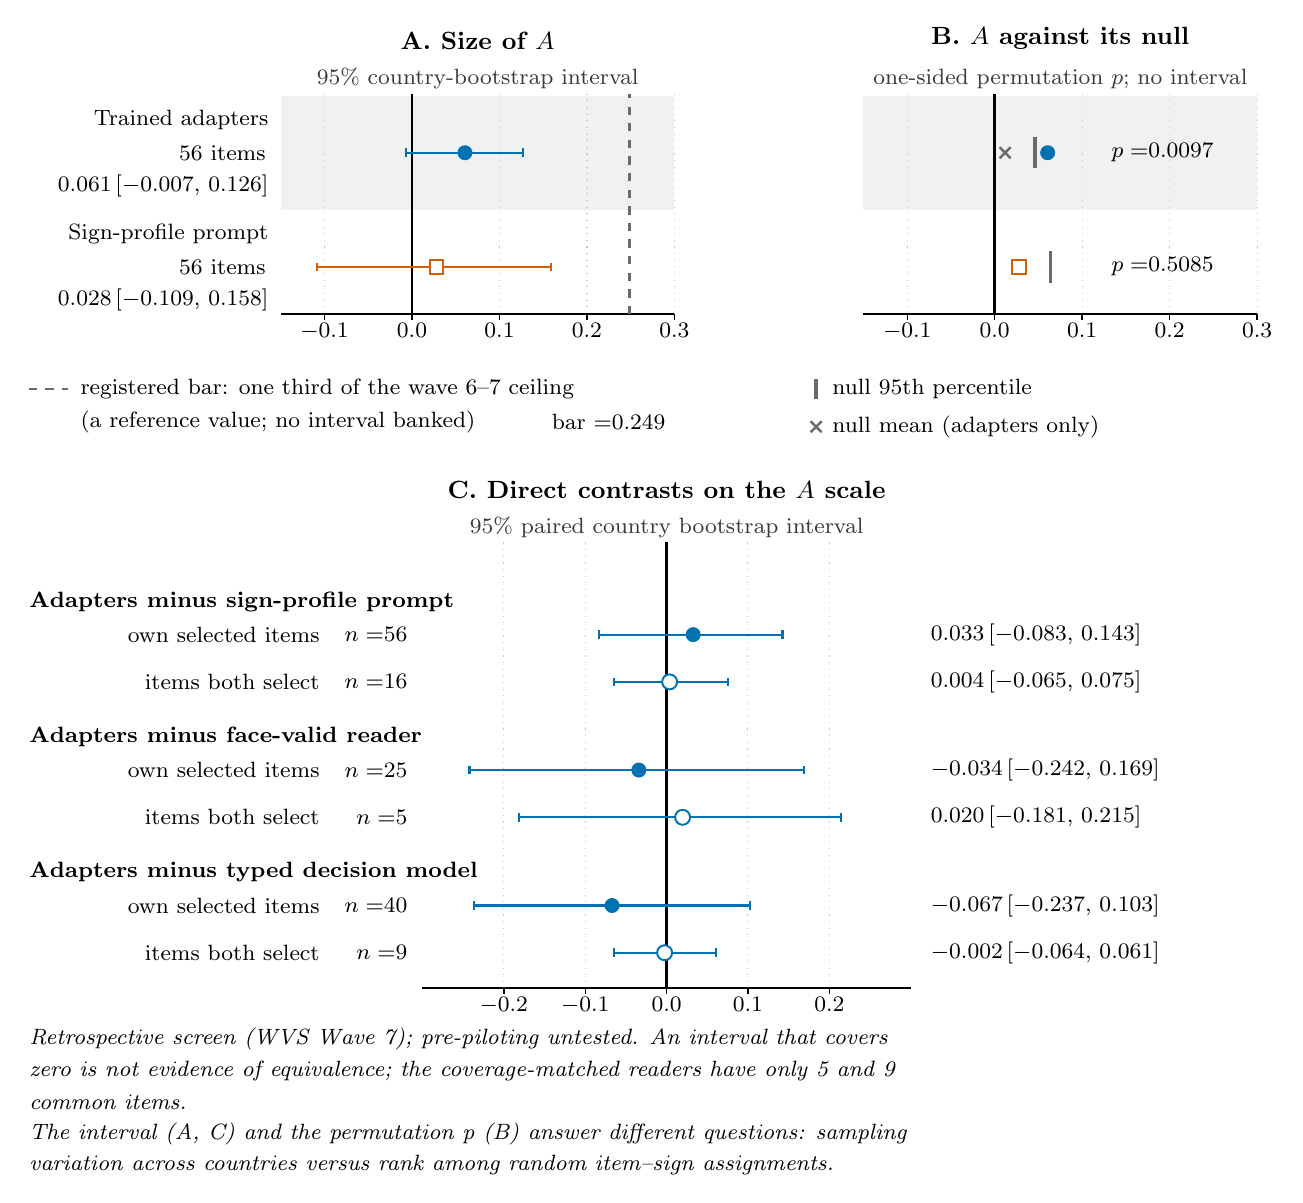
\begin{tikzpicture}[x=1cm,y=1cm,every node/.style={text=black}]
\fill[zebra] (3.200,-1.475) rectangle (8.200,-0.025);
\fill[zebra] (10.600,-1.475) rectangle (15.600,-0.025);
\setpanel{3.20000000000000017763568394002504646778106689453125}{-0.15}{11.111111}
\draw[gridc,line width=0.4pt,dotted] (3.756,0.000)--(3.756,-2.800);
\draw[black,line width=0.5pt] (3.756,-2.800)--(3.756,-2.870);
\node[anchor=north,inner sep=1pt,font=\footnotesize] at (3.756,-2.870) {$-$0.1};
\draw[gridc,line width=0.4pt,dotted] (4.867,0.000)--(4.867,-2.800);
\draw[black,line width=0.5pt] (4.867,-2.800)--(4.867,-2.870);
\node[anchor=north,inner sep=1pt,font=\footnotesize] at (4.867,-2.870) {0.0};
\draw[gridc,line width=0.4pt,dotted] (5.978,0.000)--(5.978,-2.800);
\draw[black,line width=0.5pt] (5.978,-2.800)--(5.978,-2.870);
\node[anchor=north,inner sep=1pt,font=\footnotesize] at (5.978,-2.870) {0.1};
\draw[gridc,line width=0.4pt,dotted] (7.089,0.000)--(7.089,-2.800);
\draw[black,line width=0.5pt] (7.089,-2.800)--(7.089,-2.870);
\node[anchor=north,inner sep=1pt,font=\footnotesize] at (7.089,-2.870) {0.2};
\draw[gridc,line width=0.4pt,dotted] (8.200,0.000)--(8.200,-2.800);
\draw[black,line width=0.5pt] (8.200,-2.800)--(8.200,-2.870);
\node[anchor=north,inner sep=1pt,font=\footnotesize] at (8.200,-2.870) {0.3};
\draw[black,line width=0.5pt] (3.200,-2.800)--(8.200,-2.800);
\draw[black,line width=0.9pt] (4.867,0.000)--(4.867,-2.800);
\node[anchor=south,inner sep=0pt,font=\small\bfseries,align=center] at (5.700,0.550) {A. Size of $A$};
\node[anchor=south,inner sep=0pt,font=\footnotesize,text=cS,align=center] at (5.700,0.050) {95\% country-bootstrap interval};
\setpanel{10.5999999999999996447286321199499070644378662109375}{-0.15}{11.111111}
\draw[gridc,line width=0.4pt,dotted] (11.156,0.000)--(11.156,-2.800);
\draw[black,line width=0.5pt] (11.156,-2.800)--(11.156,-2.870);
\node[anchor=north,inner sep=1pt,font=\footnotesize] at (11.156,-2.870) {$-$0.1};
\draw[gridc,line width=0.4pt,dotted] (12.267,0.000)--(12.267,-2.800);
\draw[black,line width=0.5pt] (12.267,-2.800)--(12.267,-2.870);
\node[anchor=north,inner sep=1pt,font=\footnotesize] at (12.267,-2.870) {0.0};
\draw[gridc,line width=0.4pt,dotted] (13.378,0.000)--(13.378,-2.800);
\draw[black,line width=0.5pt] (13.378,-2.800)--(13.378,-2.870);
\node[anchor=north,inner sep=1pt,font=\footnotesize] at (13.378,-2.870) {0.1};
\draw[gridc,line width=0.4pt,dotted] (14.489,0.000)--(14.489,-2.800);
\draw[black,line width=0.5pt] (14.489,-2.800)--(14.489,-2.870);
\node[anchor=north,inner sep=1pt,font=\footnotesize] at (14.489,-2.870) {0.2};
\draw[gridc,line width=0.4pt,dotted] (15.600,0.000)--(15.600,-2.800);
\draw[black,line width=0.5pt] (15.600,-2.800)--(15.600,-2.870);
\node[anchor=north,inner sep=1pt,font=\footnotesize] at (15.600,-2.870) {0.3};
\draw[black,line width=0.5pt] (10.600,-2.800)--(15.600,-2.800);
\draw[black,line width=0.9pt] (12.267,0.000)--(12.267,-2.800);
\node[anchor=south,inner sep=0pt,font=\small\bfseries,align=center] at (13.100,0.550) {B. $A$ against its null};
\node[anchor=south,inner sep=0pt,font=\footnotesize,text=cS,align=center] at (13.100,0.050) {one-sided permutation $p$; no interval};
\txt{3.050,-0.330}{Trained adapters}{east}{\footnotesize}
\lbl{SCR_A_primary}{n}{56}{}{ items}{3.050}{-0.750}{east}{none}
\lblci{SCR_A_primary}{0.061}{$-$0.007}{0.126}{3.050}{-1.170}{east}
\setpanel{3.20000000000000017763568394002504646778106689453125}{-0.15}{11.111111}
\ival{SCR_A_primary}{-0.0067258505657922735}{0.06057460871332797}{0.12648524013553836}{-0.750}{o}{cA}{solid}
\setpanel{10.5999999999999996447286321199499070644378662109375}{-0.15}{11.111111}
\pval{SCR_A_primary}{0.06057460871332797}{-0.750}{o}{cA}
\setpanel{10.5999999999999996447286321199499070644378662109375}{-0.15}{11.111111}
\draw[cG,line width=1.4pt] (12.781,-0.950)--(12.781,-0.550);
\draw[cG,line width=0.9pt] (12.329,-0.820)--(12.469,-0.680);
\draw[cG,line width=0.9pt] (12.329,-0.680)--(12.469,-0.820);
\lbl{SCR_p_perm}{value}{0.0097}{$p=$}{}{13.711}{-0.750}{west}{none}
\txt{3.050,-1.780}{Sign-profile prompt}{east}{\footnotesize}
\lbl{SP_A_primary}{n}{56}{}{ items}{3.050}{-2.200}{east}{none}
\lblci{SP_A_primary}{0.028}{$-$0.109}{0.158}{3.050}{-2.620}{east}
\setpanel{3.20000000000000017763568394002504646778106689453125}{-0.15}{11.111111}
\ival{SP_A_primary}{-0.10859510229614298}{0.027886269552101026}{0.1584453830215301}{-2.200}{q}{cB}{solid}
\setpanel{10.5999999999999996447286321199499070644378662109375}{-0.15}{11.111111}
\pval{SP_A_primary}{0.027886269552101026}{-2.200}{q}{cB}
\setpanel{10.5999999999999996447286321199499070644378662109375}{-0.15}{11.111111}
\draw[cG,line width=1.4pt] (12.976,-2.400)--(12.976,-2.000);
\lbl{SP_p_perm}{value}{0.5085}{$p=$}{}{13.711}{-2.200}{west}{none}
\setpanel{3.20000000000000017763568394002504646778106689453125}{-0.15}{11.111111}
\vref{SCR_one_third_ceiling}{0.24861871005246683}{-2.800}{0.000}{cG}
\draw[cG,dashed,line width=0.8pt] (0.0,-3.750)--(0.5,-3.750);
\txt{0.650,-3.750}{registered bar: one third of the wave 6--7 ceiling}{west}{\footnotesize}
\txt{0.650,-4.170}{(a reference value; no interval banked)}{west}{\footnotesize}
\lbl{SCR_one_third_ceiling}{value}{0.249}{bar $=$}{}{6.600}{-4.170}{west}{none}
\draw[cG,line width=1.4pt] (10.00,-3.880)--(10.00,-3.620);
\txt{10.200,-3.750}{null 95th percentile}{west}{\footnotesize}
\draw[cG,line width=0.9pt] (9.930,-4.300)--(10.070,-4.160);
\draw[cG,line width=0.9pt] (9.930,-4.160)--(10.070,-4.300);
\txt{10.200,-4.230}{null mean (adapters only)}{west}{\footnotesize}
\setpanel{5}{-0.3}{10.333333}
\draw[gridc,line width=0.4pt,dotted] (6.033,-5.700)--(6.033,-11.360);
\draw[black,line width=0.5pt] (6.033,-11.360)--(6.033,-11.430);
\node[anchor=north,inner sep=1pt,font=\footnotesize] at (6.033,-11.430) {$-$0.2};
\draw[gridc,line width=0.4pt,dotted] (7.067,-5.700)--(7.067,-11.360);
\draw[black,line width=0.5pt] (7.067,-11.360)--(7.067,-11.430);
\node[anchor=north,inner sep=1pt,font=\footnotesize] at (7.067,-11.430) {$-$0.1};
\draw[gridc,line width=0.4pt,dotted] (8.100,-5.700)--(8.100,-11.360);
\draw[black,line width=0.5pt] (8.100,-11.360)--(8.100,-11.430);
\node[anchor=north,inner sep=1pt,font=\footnotesize] at (8.100,-11.430) {0.0};
\draw[gridc,line width=0.4pt,dotted] (9.133,-5.700)--(9.133,-11.360);
\draw[black,line width=0.5pt] (9.133,-11.360)--(9.133,-11.430);
\node[anchor=north,inner sep=1pt,font=\footnotesize] at (9.133,-11.430) {0.1};
\draw[gridc,line width=0.4pt,dotted] (10.167,-5.700)--(10.167,-11.360);
\draw[black,line width=0.5pt] (10.167,-11.360)--(10.167,-11.430);
\node[anchor=north,inner sep=1pt,font=\footnotesize] at (10.167,-11.430) {0.2};
\draw[black,line width=0.5pt] (5.000,-11.360)--(11.200,-11.360);
\draw[black,line width=0.9pt] (8.100,-5.700)--(8.100,-11.360);
\node[anchor=south,inner sep=0pt,font=\small\bfseries,align=center] at (8.100,-5.150) {C. Direct contrasts on the $A$ scale};
\node[anchor=south,inner sep=0pt,font=\footnotesize,text=cS,align=center] at (8.100,-5.650) {95\% paired country bootstrap interval};
\txt{0.000,-6.450}{\textbf{Adapters minus sign-profile prompt}}{west}{\footnotesize}
\txt{3.700,-6.870}{own selected items}{east}{\footnotesize}
\lbl{SP_D_own}{n}{56}{$n=$}{}{4.850}{-6.870}{east}{none}
\setpanel{5}{-0.3}{10.333333}
\ival{SP_D_own}{-0.0833125828920078}{0.032688339161226945}{0.14255259524880806}{-6.870}{o}{cA}{solid}
\lblci{SP_D_own}{0.033}{$-$0.083}{0.143}{11.450}{-6.870}{west}
\txt{3.700,-7.470}{items both select}{east}{\footnotesize}
\lbl{SP_D_common}{n}{16}{$n=$}{}{4.850}{-7.470}{east}{none}
\setpanel{5}{-0.3}{10.333333}
\ival{SP_D_common}{-0.06495204948348372}{0.0037631428638459155}{0.0754296387941381}{-7.470}{h}{cA}{solid}
\lblci{SP_D_common}{0.004}{$-$0.065}{0.075}{11.450}{-7.470}{west}
\txt{0.000,-8.170}{\textbf{Adapters minus face-valid reader}}{west}{\footnotesize}
\txt{3.700,-8.590}{own selected items}{east}{\footnotesize}
\lbl{CMP_face_valid_D_own}{n}{25}{$n=$}{}{4.850}{-8.590}{east}{none}
\setpanel{5}{-0.3}{10.333333}
\ival{CMP_face_valid_D_own}{-0.24211281427302758}{-0.03414016762732533}{0.16872706166406723}{-8.590}{o}{cA}{solid}
\lblci{CMP_face_valid_D_own}{$-$0.034}{$-$0.242}{0.169}{11.450}{-8.590}{west}
\txt{3.700,-9.190}{items both select}{east}{\footnotesize}
\lbl{CMP_face_valid_D_common}{n}{5}{$n=$}{}{4.850}{-9.190}{east}{none}
\setpanel{5}{-0.3}{10.333333}
\ival{CMP_face_valid_D_common}{-0.18143849863495343}{0.01970706072565942}{0.21473070671106956}{-9.190}{h}{cA}{solid}
\lblci{CMP_face_valid_D_common}{0.020}{$-$0.181}{0.215}{11.450}{-9.190}{west}
\txt{0.000,-9.890}{\textbf{Adapters minus typed decision model}}{west}{\footnotesize}
\txt{3.700,-10.310}{own selected items}{east}{\footnotesize}
\lbl{CMP_jev_D_own}{n}{40}{$n=$}{}{4.850}{-10.310}{east}{none}
\setpanel{5}{-0.3}{10.333333}
\ival{CMP_jev_D_own}{-0.23700918899294768}{-0.06698794855356853}{0.10288119597809976}{-10.310}{o}{cA}{solid}
\lblci{CMP_jev_D_own}{$-$0.067}{$-$0.237}{0.103}{11.450}{-10.310}{west}
\txt{3.700,-10.910}{items both select}{east}{\footnotesize}
\lbl{CMP_jev_D_common}{n}{9}{$n=$}{}{4.850}{-10.910}{east}{none}
\setpanel{5}{-0.3}{10.333333}
\ival{CMP_jev_D_common}{-0.06437316693682472}{-0.0024255192718040247}{0.06102420665810506}{-10.910}{h}{cA}{solid}
\lblci{CMP_jev_D_common}{$-$0.002}{$-$0.064}{0.061}{11.450}{-10.910}{west}
\txt{0.000,-12.010}{Retrospective screen (WVS Wave 7); pre-piloting untested. An interval that covers}{west}{\footnotesize\itshape}
\txt{0.000,-12.410}{zero is not evidence of equivalence; the coverage-matched readers have only 5 and 9}{west}{\footnotesize\itshape}
\txt{0.000,-12.810}{common items.}{west}{\footnotesize\itshape}
\txt{0.000,-13.210}{The interval (A, C) and the permutation p (B) answer different questions: sampling}{west}{\footnotesize\itshape}
\txt{0.000,-13.610}{variation across countries versus rank among random item--sign assignments.}{west}{\footnotesize\itshape}
\end{tikzpicture}
\end{document}
